\documentclass[../main.tex]{subfiles}
\graphicspath{{\subfix{../images/}}}



\begin{document}
% Include more details on all aspects in Section 2 if they can be useful for the development team

\subsection{External Interface Requirements}

\subsubsection{User Interfaces}
The eMall program consists in a mobile application compatible with the iOS and the Android operative systems. The application is designed to be used by both Drivers and Operators, and the user interface of the application is supposed to be simple to understand (e.g. functionalities can be accessed through clicking on common icons) and user-friendly, in order to maximize the usability and the user experience.

\subsubsection{Hardware Interfaces}
The hardware interface required to access to the eMall system is a working device (a mobile phone or a tablet) with internet connection that can successfully install the application. It must have fundamental sensors such as GPS and Bluetooth: the first is used for determining the location of the User and the second for the connection between the vehicle and the driver’s device.

\subsubsection{Software Interfaces}
The application makes use of an external API for geo-localisation. It provides a map for Drivers to identify their actual position and the charging stations nearby, making the interaction more explicit. In addition to this, it uses the Bluetooth API to connect to the Driver's vehicle in order to retrieve useful data for the system. 
\\
\\
For what concerns the server side of the application, the system requires the implementation of a DBMS to store the data.

\subsubsection{Communication Interfaces}
Many functionalities offered by the system relies on the communication with other services. Thanks to external APIs, e-Mall employs different interfaces: 

\begin{itemize}
    \item \textbf{Retrieval of data of a charging station}\\
    The interface is able to respond with an overview on the status a specific charging station, this is retrieved through the charging station's unique identification number. 
    \item \textbf{Retrieval of data on DSOs}\\
    The interface is able to retrieve a list of available DSOs with the information they published. In this way the operators can acquire energy from any of them for the selected charging station. 
    \item \textbf{Retrieval of map information}\\
    The eMall system provides a map for users to visualise their actual position and the available charging stations near them. In this case we need to interface with an external API which offers map and geolocation services. 
    \item \textbf{Retrieval of vehicle data}\\
    The interface is able to retrieve relevant information about the user's actual guiding vehicle, such as its battery status. This is also made possible with an external API. 
    
\end{itemize}



\subsection{Functional Requirements}
% Definition of use case diagrams, use cases and associated sequence/activity diagrams, and mapping on requirements

\subsubsection{Use cases}
In this subsection, the main use cases of the system are reported.
\\
\\
U1. Driver Registration
\vspace{-1em}
\begin{center}
\begin{longtable}[\textwidth]{| l | p{10cm} | } 
\hline
Actor & Driver \\
\hline
Entry condition & The driver have not registered an account yet, and he is on the Login page of the application \\
\hline
Event flow & {
\vspace{-1em}
\begin{enumerate}
\itemsep0em
    \item The driver clicks on the "Register" button in the Login page
    \item The driver inputs his name and surname, the email address, and the password in the registration form
    \item The driver ticks the checkbox to authorize the use of personal data
    \item The driver clicks on the "Submit" button
    \item The system processes the submitted information
\end{enumerate}
\vspace{-0.5em}
\hline
Exit condition & A new account is created for the driver and a success message is shown \\
\hline
Exceptions &  {
\vspace{-1.5em}
\begin{enumerate}
\itemsep0em
    \item The system shows an error message if the driver does not fill all the fields when submitting the form\vspace{-0.3em}
    \item The system shows an error message if the input data is invalid (e.g. the email address is already linked to another account)\vspace{-0.3em}
\end{enumerate}
\vspace{-1em}}
\hline
\end{longtable}

\end{center}
\vspace{1.5em}
\\
\\
U2. User Login
\vspace{-1em}
\begin{center}
\begin{longtable}[\textwidth]{| l | p{10cm} | } 
\hline
Actor & User (Driver or Operator) \\
\hline
Entry condition & The user has a registered account, and he is on the Login page of the application \\
\hline
Event flow & {
\vspace{-1em}
\begin{enumerate}
\itemsep0em
    \item The user clicks on the "Login" button in the Login page
    \item The driver inputs his email address and the password in the login form
    \item The driver clicks on the "Submit" button
    \item The system processes the submitted information
\end{enumerate}
\vspace{-0.5em}}
\hline
Exit condition & The user is logged in, and he is redirected to the Main page\\
\hline
Exceptions &  {
\vspace{-1.5em}
\begin{enumerate}
\itemsep0em
    \item The system shows an error message if the driver does not fill all the fields when submitting the form
    \item The system shows an error message if the input data is invalid (wrong email / password combination)
\end{enumerate}
\vspace{-1em}}
\hline
\end{longtable}
\end{center}
\\
\\
\newpage
U3. Add a vehicle to the profile
\vspace{-1em}
\begin{center}
\begin{longtable}[\textwidth]{| l | p{10cm} | } 
\hline
Actor & Driver \\
\hline
Entry condition & The driver is logged in and he is on the Main page of the application \\
\hline
Event flow & {
\vspace{-1em}
\begin{enumerate}
\itemsep0em
    \item The driver clicks on the "Profile" button in the Main page
    \item The driver selects the option to add a vehicle to his personal profile
    \item The system shows the form for adding a vehicle
    \item The driver inputs the required data, such as the vehicle's plate number and the owner
    \item The driver clicks on the "Confirm" button
    \item The system processes the submitted information
\end{enumerate}
\vspace{-0.5em}}
\hline
Exit condition & The vehicle is successfully added to the driver's profile, and he can book a charge for it now \\
\hline
Exceptions & The system shows an error message if the input data is invalid or missing 
\hline
\end{longtable}
\end{center}
\vspace{1.5em}
\\
\\
U4. Visualize charging stations nearby
\vspace{-1em}
\begin{center}
\begin{longtable}[\textwidth]{| l | p{10cm} | } 
\hline
Actor & Driver \\
\hline
Entry condition & The driver has a registered account, and he is logged in \\
\hline
Event flow & {
\vspace{-1em}
\begin{enumerate}
\itemsep0em
    \item The driver is redirected to the Main page of the application
    \item The system shows the map with the charging stations located in the area
    \item The driver selects a charging station
    \item The system redirects the driver to the charging station's status page
\end{enumerate}
\vspace{-0.5em}}
\hline
Exit condition & The charging station's status is shown \\
\hline
\end{longtable}
\end{center}
\\
\\
\newpage
U5. Book a charge
\vspace{-1em}
\begin{center}
\begin{longtable}[\textwidth]{| l | p{10cm} | } 
\hline
Actor & Driver \\
\hline
Entry condition & The driver has a registered account, he is logged in and he is at the Main page of the application \\
\hline
Event flow & {
\vspace{-1em}
\begin{enumerate}
\itemsep0em
    \item The driver selects a charging station from the map or from the list displayed in the Main page 
    \item The system shows the status of the selected charging station and the available charging options
    \item The driver selects the desired charging socket type
    \item The driver selects a time slot from the list
    \item The driver selects the vehicle he wants to charge
    \item The driver clicks on the "Confirm" button
    \item The system processes the submitted information
    \item The system shows the summary of the operation
\end{enumerate}
\vspace{-0.5em}}
\hline
Exit condition & The driver successfully makes a reservation, which is added to his booking history\\
\hline
Exceptions & {
\vspace{-1.5em}
\begin{enumerate}
\itemsep0em
    \item The system shows an error message if the data provided by the driver is invalid or missing
    \item The system shows an error message if the chosen slot is not longer available at the moment of the form submission
\end{enumerate}
\vspace{-1em}}
\hline
\end{longtable}
\end{center}
\\
\\
\newpage
U6. Start charging at the station
\vspace{-1em}
\begin{center}
\begin{longtable}[\textwidth]{| l | p{10cm} | } 
\hline
Actor & Driver \\
\hline
Entry condition & The driver is logged in, he has already booked a charge and he arrives at the charging station in time \\
\hline
Event flow & {
\vspace{-1em}
\begin{enumerate}
\itemsep0em
    \item The driver checks the charging socket from his reservation summary
    \item The driver authenticates at the correct charging column's display with the code shown on his mobile device
    \item The system verifies the identity of the driver
    \item The driver plugs the vehicle in
    \item The system verifies the vehicle's status and locks the vehicle
    \item The driver confirms the starting of the charge on the display
    \item The system shows the charging operation summary on the display
\end{enumerate}
\vspace{-0.5em}}
\hline
Exit condition & The vehicle starts charging\\
\hline
Exceptions &  {
\vspace{-1.5em}
\begin{enumerate}
\itemsep0em
    \item The display shows an error message if the driver does not authenticate correctly
    \item The display shows an error message if the vehicle is not correctly identified
\end{enumerate}
\vspace{-1em}}
\hline
\end{longtable}
\end{center}
\\
\\
\newpage
U7. End charging
\vspace{-1em}
\begin{center}
\begin{longtable}[\textwidth]{| l | p{10cm} | } 
\hline
Actor & Driver \\
\hline
Entry condition & The driver's vehicle has finished to charge at the station \\
\hline
Event flow & {
\vspace{-1em}
\begin{enumerate}
\itemsep0em
    \item The system notifies the driver about the status of the vehicle
    \item The driver arrives at the charging station and authenticates at the charging column
    \item The system verifies the identity of the driver
    \item The system shows the operation summary and the amount to pay through the charging column's display
    \item The driver pays for the operation using cash or credit card
    \item The system handles the payment
\end{enumerate}
\vspace{-0.5em}}
\hline
Exit condition & The system unlocks the vehicle, and the driver picks it up \\
\hline
Exceptions &  {
\vspace{-1.5em}
\begin{enumerate}
\itemsep0em
    \item The display shows an error message if the driver does not authenticate correctly
    \item The display shows an error message if the payment fails
\end{enumerate}}
\vspace{-1em}
\hline
\end{longtable}
\end{center}
\\
\\
\newpage
U8. Send charging suggestions
\vspace{-1em}
\begin{center}
\begin{longtable}[\textwidth]{| l | p{10cm} | } 
\hline
Actor & Driver\\
\hline
Entry condition & The driver is logged in, and the system detects the vehicle's low battery status \\
\hline
Event flow & {
\vspace{-1em}
\begin{enumerate}
\itemsep0em
    \item The system checks the calendar of the driver to get information about his schedule
    \item The system checks the navigation path of the driver
    \item The system finds the charging stations near to the path of the driver
    \item The system checks the selected stations' availability according to the driver's schedule
    \item The system finds the suitable charging station and notifies the driver
\end{enumerate}
\vspace{-0.5em}}
\hline
Exit condition & The driver receives the suggestion of the system\\
\hline
\end{longtable}
\end{center}
\\
\\
\newpage
U9. Define a special offer
\vspace{-1em}
\begin{center}
\begin{longtable}[\textwidth]{| l | p{10cm} | } 
\hline
Actor & Operator \\
\hline
Entry condition & The operator is logged in and he is at the Main page of the application \\
\hline
Event flow & {
\vspace{-1em}
\begin{enumerate}
\itemsep0em
    \item The operator selects the charging station he wants to manage from the list reported in the Main page
    \item The operator selects the option to make a new offer
    \item The system displays a form for the creation of the offer
    \item The operator defines the offer's type and price
    \item The operator selects the starting date and the end date of the offer
    \item The operator clicks on the "Submit" button
    \item The system processes the submitted information and shows the operation summary
    
\end{enumerate}
\vspace{-0.5em}}
\hline
Exit condition & The new offer is published successfully \\
\hline
Exceptions & {
\begin{enumerate}
\itemsep0em
    \item The system shows an error message if the chosen combination of starting date and end date is invalid
    \item The system shows an error message if the value of price is invalid
\end{enumerate}} \\
\hline
\end{longtable}
\end{center}
\\
\\
\newpage
U10. Modify the energy source used for charging
\vspace{-1em}
\begin{center}
\begin{longtable}[\textwidth]{| l | p{10cm} | } 
\hline
Actor & Operator \\
\hline
Entry condition & The operator is logged in and he is at the Main page of the application \\
\hline
Event flow & {
\vspace{-1em}
\begin{enumerate}
\itemsep0em
    \item The operator selects the charging station he wants to manage from the list
    \item The system displays the current status of the chosen charging station
    \item The operator selects to change the energy source used for charging
    \item The system shows a list of available options
    \item The operator chooses an option and clicks on the "Confirm" button
    \item The system processes the submitted information
\end{enumerate}
\vspace{-0.5em}}
\hline
Exit condition & The current energy source is modified \\
\hline
Exceptions & The system shows an error message if the option turns to be invalid at the moment of the submission \\
\hline
\end{longtable}
\end{center}
\\
\\
\newpage
U11. Modify the charging price
\vspace{-1em}
\begin{center}
\begin{longtable}[\textwidth]{| l | p{10cm} | } 
\hline
Actor & Operator \\
\hline
Entry condition & The operator is logged in and he is at the Main page of the application \\
\hline
Event flow & {
\vspace{-1em}
\begin{enumerate}
\itemsep0em
    \item The operator selects the charging station from the list
    \item The system displays the current status of the chosen charging station
    \item The operator selects the type of charge he wants to modify the price
    \item The operator defines the new charging cost
    \item The operator clicks on "Submit" button
    \item The system processes the submitted information
\end{enumerate}
\vspace{-0.5em}}
\hline
Exit condition & The price is modified and the page is refreshed to show the updated information \\
\hline
Exceptions & The system shows an error message if the input data is invalid (wrong format) \\
\hline
\end{longtable}
\end{center}
\\
\\
\newpage
U12. Acquire energy from DSOs
\vspace{-1em}
\begin{center}
\begin{longtable}[\textwidth]{| l | p{10cm} | } 
\hline
Actor & Operator \\
\hline
Entry condition & The operator is logged in and he is at the Main page of the application \\
\hline
Event flow & {
\vspace{-1em}
\begin{enumerate}
\itemsep0em
    \item The operator clicks on the "Acquire energy" button
    \item The system collects the list of offers published by the DSOs and displays it
    \item The operator selects an available option
    \item The operator decides the quantity of energy he wants to acquire and the related charging station
    \item The system shows the operation summary
    \item The operator clicks on the "Submit" button
    \item The system processes the submitted information
\end{enumerate}
\vspace{-0.5em}}
\hline
Exit condition & The new offer is published successfully \\
\hline
Exceptions & The system shows an error message the input data is invalid
\hline
\end{longtable}
\end{center}
\vspace{0.5em}
\subsubsection{Use cases Diagrams}
\hspace{1em}1. Unregistered Driver
\begin{figure}[H]
    \centering
    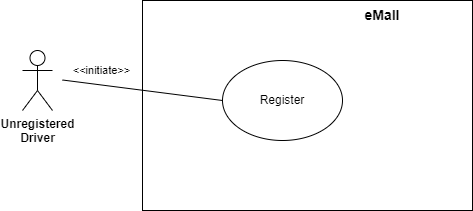
\includegraphics[width=0.8\textwidth]{usecases/uc_unregistered.png}
    \caption{Use case diagram for an unregistered driver}
    \label{fig:unregistered}
\end{figure}
\\
\\
2. Authenticated Driver
\begin{figure}[H]
    \centering
    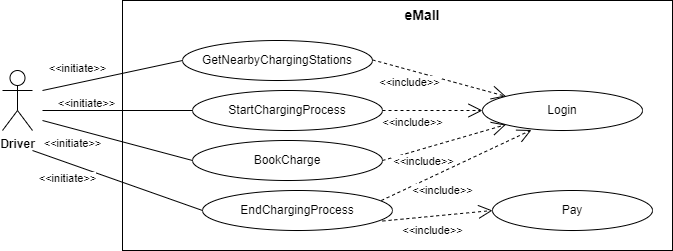
\includegraphics[width=0.9\textwidth]{usecases/uc_driver.png}
    \caption{Use case diagram for an authenticated driver}
    \label{fig:driver}
\end{figure}
\\
\\
3. Authenticated Operator
\begin{figure}[H]
    \centering
    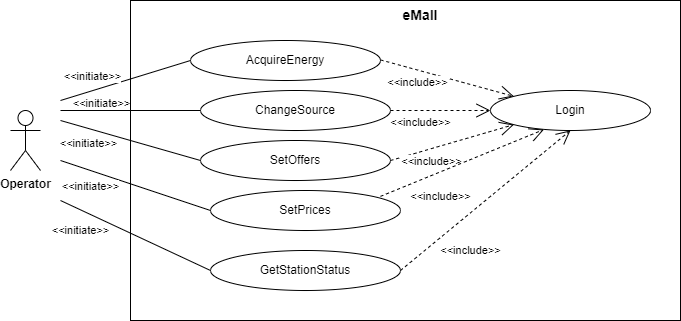
\includegraphics[width=0.9\textwidth]{usecases/uc_operator.png}
    \caption{Use case diagram for an authenticated operator}
    \label{fig:operator}
\end{figure}


\subsubsection{Sequence Diagrams}
In this section, the corresponding sequence diagrams for the use cases are presented. Overall, we consider that the actor has been logged in all cases except for “Registration” and “Login” cases.
\\
\\
\newpage
1. Register
\begin{figure}[H]
    \centering
    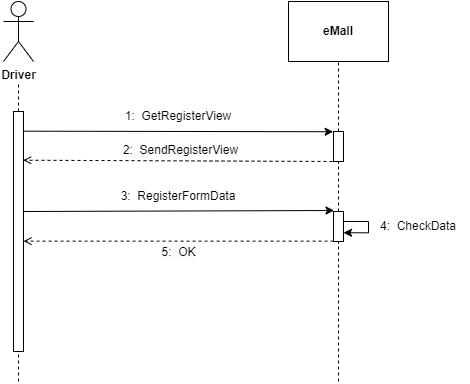
\includegraphics[width=0.65\textwidth]{sequences/sd_register.png}
    \caption{Sequence diagram for a Driver's Registration process}
    \label{fig:register}
\end{figure}

2. Login
\begin{figure}[H]
    \centering
    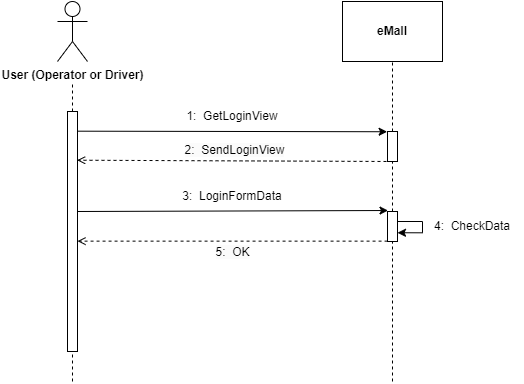
\includegraphics[width=0.65\textwidth]{sequences/sd_login.png}
    \caption{Sequence diagram for the Login process}
    \label{fig:login}
\end{figure}

3. Get charging stations
\begin{figure}[H]
    \centering
    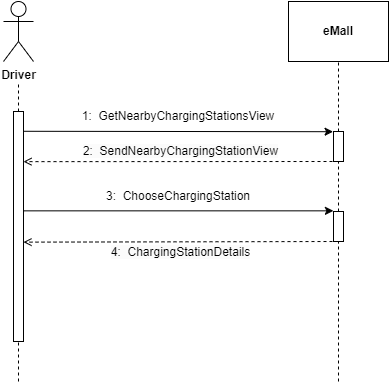
\includegraphics[width=0.45\textwidth]{sequences/sd_getChargingStations.png}
    \caption{Sequence diagram for the process when a driver is searching for a nearby charging station}
    \label{fig:getstations}
\end{figure}

4. Book a charge
\begin{figure}[H]
    \centering
    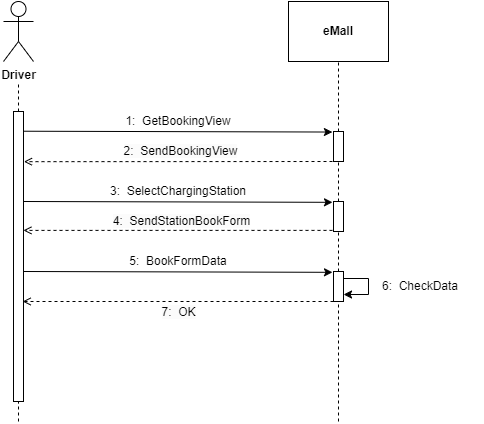
\includegraphics[width=0.6\textwidth]{sequences/sd_booking.png}
    \caption{Sequence diagram for booking a charge by a driver}
    \label{fig:booking}
\end{figure}

5. Start a charging process
\begin{figure}[H]
    \centering
    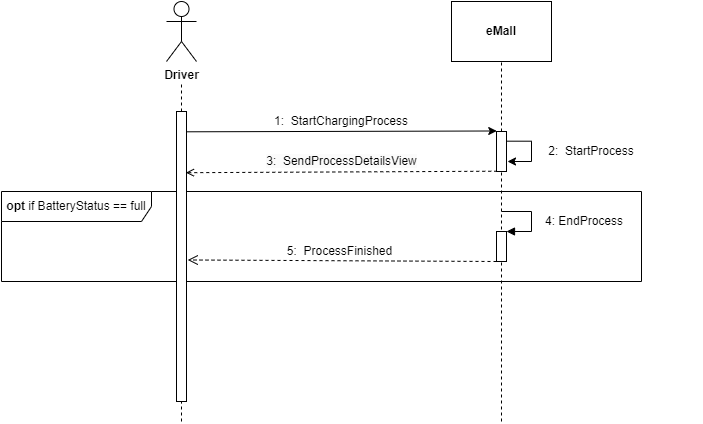
\includegraphics[width=0.75\textwidth]{sequences/sd_startCharge.png}
    \caption{Sequence diagram for starting a charging process. The possibility of getting the battery full is also presented.}
    \label{fig:startCharge}
\end{figure}

6. End a charging process
\begin{figure}[H]
    \centering
    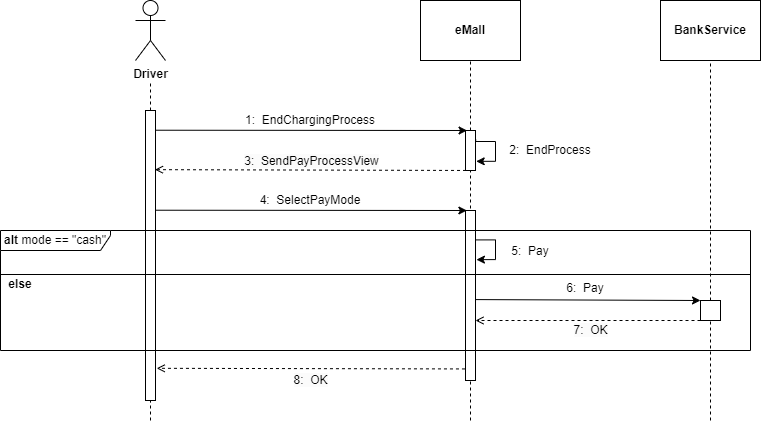
\includegraphics[width=0.75\textwidth]{sequences/sd_endCharge.png}
    \caption{Sequence diagram for ending a charging process. The process of pay the charge is also included in the diagram and different methods of payment (Cash or Credit Card) are also presented.}
    \label{fig:endCharge}
\end{figure}

7. Get a charging station’s status
\begin{figure}[H]
    \centering
    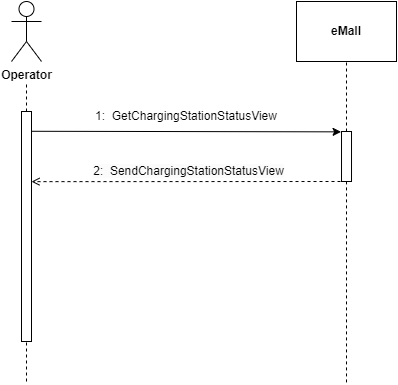
\includegraphics[width=0.45\textwidth]{sequences/sd_getStatus.png}
    \caption{Sequence diagram for getting a charge station’s status by an operator}
    \label{fig:getStatus}
\end{figure}

8. Set an offer
\begin{figure}[H]
    \centering
    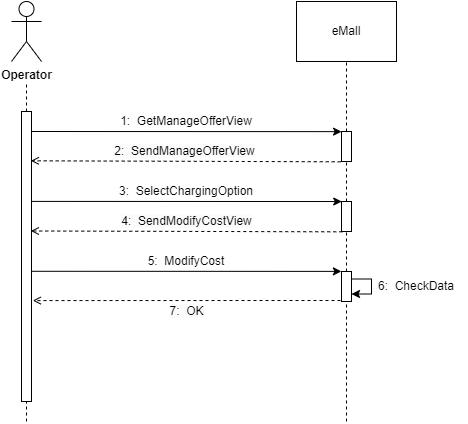
\includegraphics[width=0.65\textwidth]{sequences/sd_offer.png}
    \caption{Sequence diagram for setting a special offer by an operator}
    \label{fig:offer}
\end{figure}

9. Acquire energy
\begin{figure}[H]
    \centering
    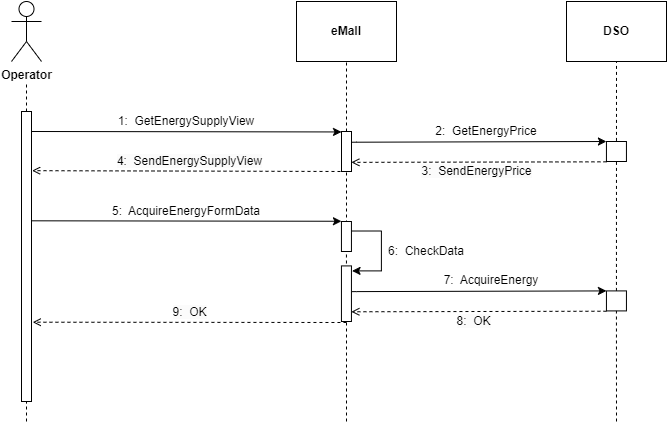
\includegraphics[width=0.9\textwidth]{sequences/sd_acquire.png}
    \caption{Sequence diagram for acquiring energy from external DSOs by an operator. The interactions between the system and a generic DSO are presented.}
    \label{fig:acquire}
\end{figure}

\newpage
10. Change source
\begin{figure}[H]
    \centering
    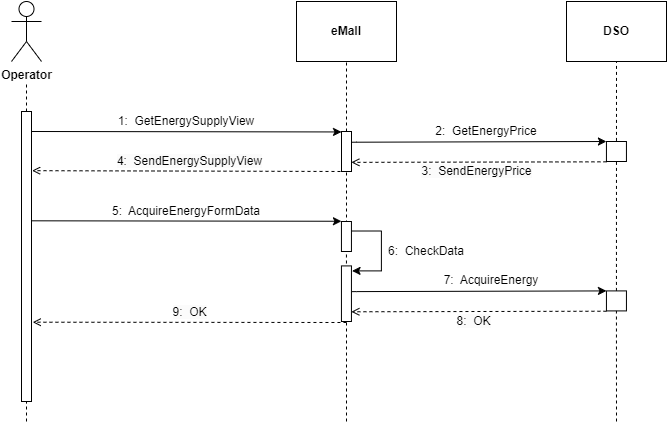
\includegraphics[width=0.9\textwidth]{sequences/sd_acquire.png}
    \caption{Sequence diagram for acquiring energy from external DSOs by an operator. The interactions between the system and a generic DSO are presented.}
    \label{fig:acquire}
\end{figure}


\subsubsection{List of Functional Requirements}

\begin{center}
\begin{longtable}{| c | p{12cm} | } 
\hline
\textbf{Identifier} & \textbf{Description} \\
\hline
R1 & The system shall allow an unregistered Driver to register and create an account \\ 
\hline
R2 & The system shall allow a registered Driver to log into his account\\
\hline
R3 & The system shall allow a registered Driver to delete his account\\
\hline
R4 & The system shall allow a registered Driver to add one or more vehicles to his account\\
\hline
R5 & The system shall allow a registered Driver to delete one or more vehicles from his account\\
\hline
R6 & The system shall allow a registered Driver to book a charging slot of a station for a certain time frame\\
\hline
R7 & The system shall allow a registered Driver to acquire information of a selected charging station\\
%\hline
%R8 & The system shall allow a registered Driver to book a charge in a charging station in a certain time frame\\
\hline
R8 & The system shall allow a registered Driver to visualise the details of his charging process \\
\hline
R9 & The system shall allow a registered Driver to visualize the current offers of charging stations\\
\hline
R10 & The system shall allow a registered Driver to pay for the obtained service through an external API\\
\hline
R11 & The system shall allow a registered Driver to cancel a reservation \\
\hline
R12 & The system shall not allow a registered Driver to book for a charge when he has already a reservation\\
\hline
R13 & The system shall allow a registered Driver to know about his actual position and nearby charging stations through an external API\\
\hline
R14 & The system shall allow an Operator working for the CPO to log into his account
\\
\hline
R15 & The system shall allow a registered Operator to create an offer to the charging station managed by him
\\
\hline
R16 & The system shall allow a registered Operator to modify the charging source of the charging station managed by him
\\
\hline
R17 & The system shall allow a registered Operator to modify the price of the energy of a charging station managed by him
\\
\hline
R18 & The system shall allow a registered Operator to check the status of the charging station managed by him
\\
\hline
R19 & The system shall allow a registered Operator to visualise data provided by DSOs
\\
\hline
R20 & The system shall allow a registered Operator to choose from which DSO to acquire energy
\\
\hline
R21 & The system must be able to decide automatically where to get energy for charging
\\
\hline
R22 & The system must be able to notify the Driver when the charging process starts
\\
\hline
R23 & The system must be able to notify the Driver when the charging process ends
\\
\hline
R24 & The system must be able to suggest the Driver to charge the vehicle, the suggestion is based on information retrieved through external APIs \\
\hline
R25 & The system must be able to notify user in case of exceptions
\\
\hline
R26 & The system must be able to notify user on successful actions
\\
\hline
R27 & The system must be able to retrieve a map through an external API
\\
\hline
\end{longtable}
\end{center}



\subsection{Mapping on Goals}
The following traceability matrix summarizes the mapping between the goals and the requirements which can guarantee the achievement of the goals under some domain assumptions. 

\begin{center}
\begin{longtable}{| c | p{3cm} | p{6cm} | p{2.5cm} |} 
 \hline
 \textbf{Goals} & \textbf{Assumptions} &\textbf{Requirements} & \textbf{Use Cases} \\
 \hline
 G1 & D8, D9 & R1, R2, R7, R9, R13, R25, R26, R27 & U1, U2, U4 \\
 \hline
 G2 & D1, D2 & R1, R2, R4, R6, R7, R9, R11, R12, R25, R26 & U1, U2, U3, U4, U5\\
 \hline
 G3 & D2, D3, D4, D8 & R1, R2, R4, R6, R7, R8, R22, R25, R26, R27 & U5, U6, U7 \\
 %\hline NO G4 & D9, D10 & C \\
 \hline
 G4 & D6, D8 & R1, R2, R4, R5, R6, R8, R9, R10, R23, R25, R26 & U7 \\
 \hline
 G5 & D1, D5, D9 & R1, R2, R4, R5, R7, R9, R13, R24 
 & U2, U3, U8\\
 %\hline NO G7 & D7, D10 & C \\
 %\hline NO G8 & D9, D10 & C \\
 %\hline NO G9 & D8, D10 & C \\
 \hline
 G6 & D8 & R14, R18, R20, R25, R26 & U2, U10 \\
 \hline
 G7 & D8 & R14, R16, R18, R21, R25, R26 & U2, U9, U11 \\
 \hline
 G8 & D7, D8 & R14, R15, R17, R18, R19, R25, R26 & U2, U12 \\
 \hline


 \end{longtable}
 \end{center}

\newpage
\subsection{Design Constraints}

\subsubsection{Non-Functional Requirements}
\begin{center}
\begin{longtable}{| c | p{12cm} | } 
\hline
\textbf{Identifier} & \textbf{Description} \\
\hline

NR1 & The system has to provide a feedback in 5 seconds
\\
\hline
NR2 & The system must tolerate slow internet connection
\\
\hline
NR3 & Failures in the system must be fixed within 2 hours
\\
\hline
NR4 & The system should be available 99\% of the time
\\
\hline
NR5 & The system must be easy to understand and to use
\\
\hline
NR6 & The system must provide an user-friendly user interface
\\
\hline
NR7 & The system must support different operating systems including iOS, Android and HarmonyOS (Versions ?)
\\
\hline
NR8 & The system must support different devices in particular smartphone and tablet with different screen sizes 
\\
\hline
NR9 & The hardware on which the system runs must have sensors in particular GPS and Bluetooth
\\
\hline
NR10 & The device while running the system must be connected to internet
\\
\hline
NR11 & The system should never allow unregistered user to use its functionalities
\\
\hline
NR12 & The system must protect sensitive information provided by users
\\
\hline
NR13 & personal data and sensitive personal data collected from the system shall be treated in compliance with GDPR 
\\
\hline
NR14 & The system must not let unauthorised users to access sensitive information
\\
\hline
NR15 & When making use of external APIs, the system must follow their regulation and guidelines
\\
\hline
NR16 & The system should be easily modifiable for future improvement and adaptation to the evolving requirements or changes in the environment
\\
\hline
\end{longtable}
\end{center}

\subsubsection{Standards compliance}
All users' personal data is treated in compliance with the GDPR (NR13). The employment of external APIs must be done following regulations and guidelines (NR15).

\subsubsection{Hardware limitations}
The device on which the application runs can be a smartphone or a tablet (NR8). It must be able to connect to Internet (NR10) and it must have the required sensors, in particular GPS and Bluetooth (NR9) for the correct working of the application. 

% \subsubsection{Any other constraint}


\subsection{Software System Attributes}

\subsubsection{Reliability}
The system should be highly reliable, and running without failure most of the time. If failures happen, it should be able to recover quickly (NR3). To achieve this, regular maintenance should be done.
\\
Since the system relies also on several external API which do not depend on our system, it must not completely fail when one of those fail. 

\subsubsection{Availability}
The aimed availability for the system is 99\%: in fact, the system must be available and running most of the time, especially during the business hours (NR2, NR3, NR4), although it is not a big issue for the system to have some short downtime. In the case that a Driver should book for a charge, if he is not in a rush, he can simply do it later. If the system is down while the driver is charging, he can complete the charging process and pay for the service later. 

\subsubsection{Security}
The information that the system is handling can be either public or sensitive. The latest need to be protected (NR11, NR12, NR13, NR14, NR15). To do so, the system can make use of different approaches such as limiting the access by setting different authorisation level so that unauthorised users are denied to access. In the case of password, it is possible to scramble it through encryption algorithm, so that it is unreadable by unauthorised ones.

\subsubsection{Maintainability}
The system should be easily modifiable for future improvement and adaptation to the evolving requirements or changes in the environment (NR16). In order to achieve this, it is important to keep in line the document while realizing the application. Moreover, it is fundamental to re-use design patterns which helps to prevent subtle issues that can cause major problems, and to improve code readability.


\subsubsection{Portability}
The eMall application should be installed on a device to be used. The User interface and functionalities of the system should work well on different screen sizes of different devices, mobile phone or tablet, with different operating systems such as iOS, Android and HarmonyOS (NR7, NR8).


% \subsection{Other Requirements}










\end{document}
